%%%%&latex
\documentclass[12pt]{article}
\usepackage{amsmath}
\usepackage{graphicx}
\usepackage{psfrag,epsf,enumerate}
\usepackage{enumerate}
\usepackage{natbib}
\usepackage{url} % not crucial - just used below for the URL

\usepackage{amssymb, qtree, bm, multirow, textcmds, siunitx,paralist}
\usepackage{mathrsfs, float, booktabs,todonotes,amsthm}
\usepackage[bb=boondox]{mathalfa}
\usepackage{tikz}
\usetikzlibrary{arrows,positioning,shapes,fit,calc}
\usepackage{amsfonts}
\usepackage[section]{placeins}
\usepackage{amsthm,algorithm,algorithmicx,algpseudocode}
%\pdfminorversion=4
% NOTE: To produce blinded version, replace "0" with "1" below.
\newcommand{\blind}{1}

% DON'T change margins - should be 1 inch all around.
\addtolength{\oddsidemargin}{-.5in}%
\addtolength{\evensidemargin}{-.5in}%
\addtolength{\textwidth}{1in}%
\addtolength{\textheight}{1in}%
\addtolength{\topmargin}{-.8in}%


\begin{document}


%\section{Forecasting Australian domestic tourism flows}\label{sec:Application}


\begin{figure}
	\centering
	\small
    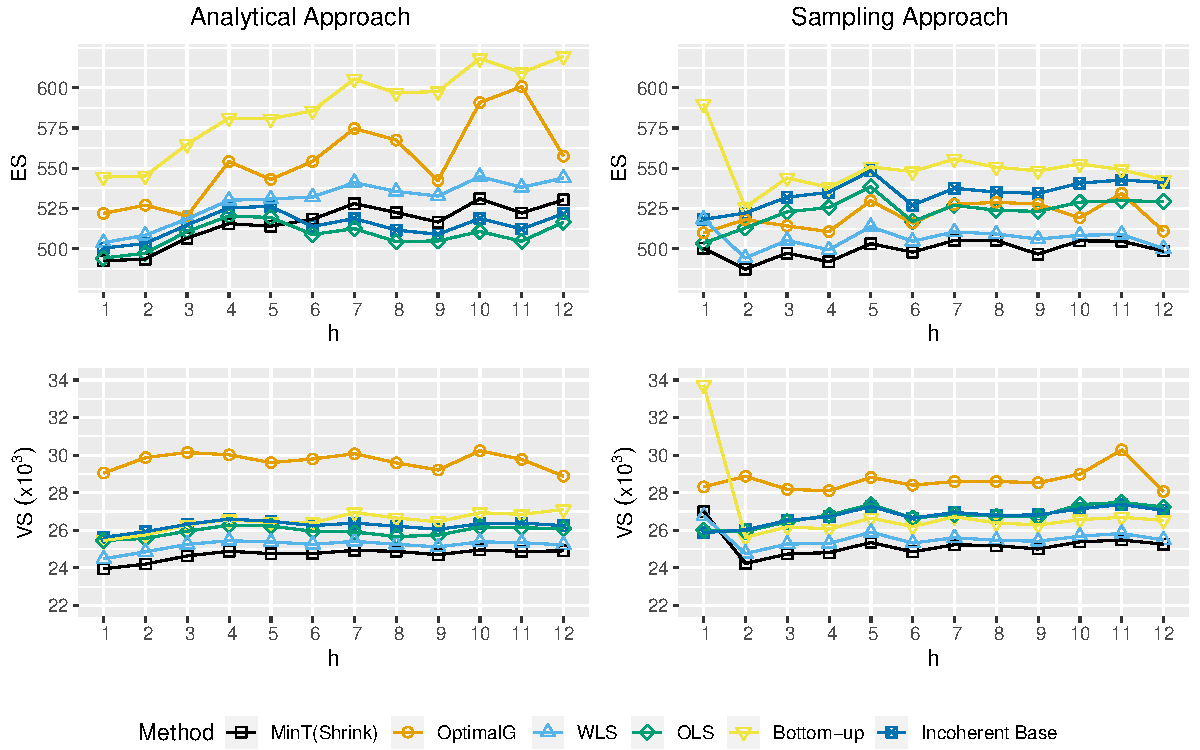
\includegraphics[width=.95\textwidth]{RawScore_Overall.pdf}
	\caption{Energy and variogram scores for multivariate predictive distributions across the entire hierarchy. A lower (higher) score indicates a more (less) accurate forecast. Results from the analytic approach assuming Gaussian incoherent base forecasts are presented on the left while results from the non-parametric approach are presented on the right.} \label{fig:Scores_Overall}
\end{figure}


\begin{figure}
	\centering
	\small
    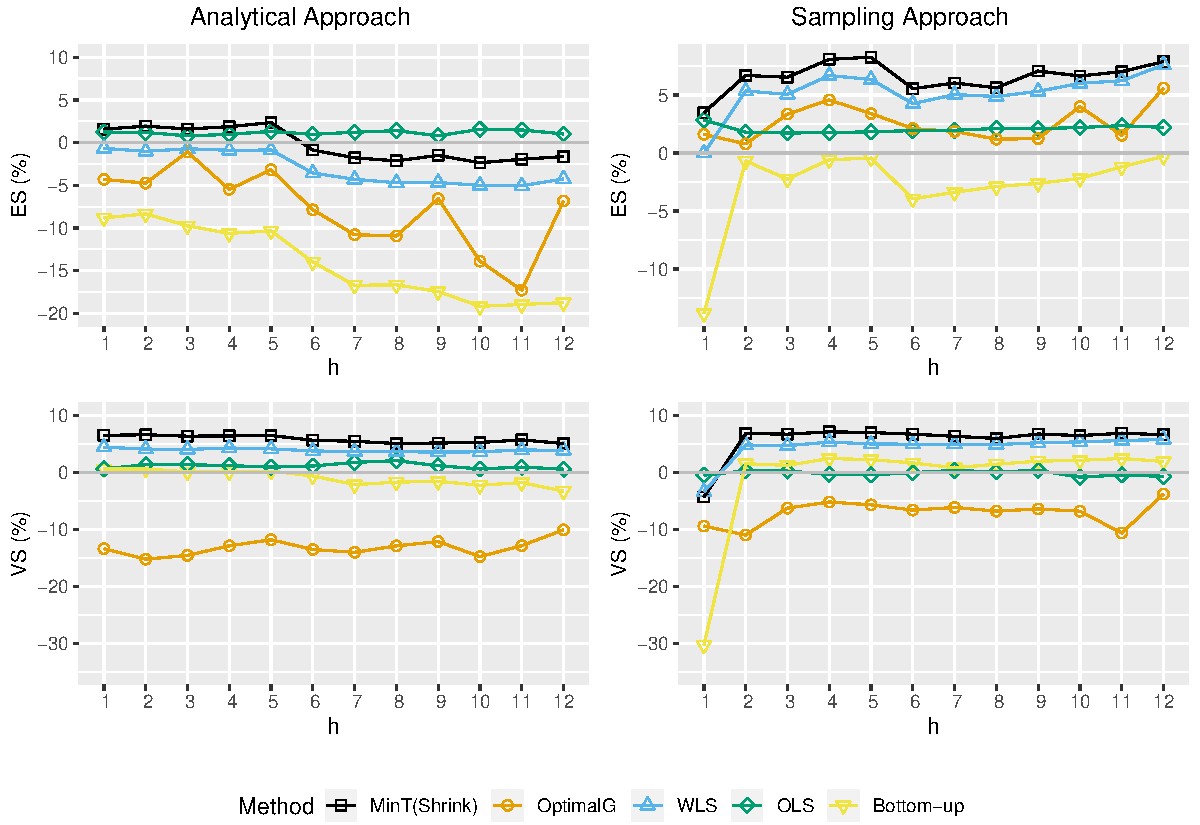
\includegraphics[width=.95\textwidth]{SkillScore_Overall.pdf}
	\caption{Skill scores (\%) relative to incoherent base forecasts, across the entire Australian tourism hierarchy based on energy score (on the left) and variogram score (on the right). A higher (lower) score indicates a gain (loss) in forecast accuracy relative to the incoherent base forecasts. The results are for the analytic solution assuming Gaussian incoherent base forecasts.} \label{fig:SkillScores_Overall}
\end{figure}


\begin{figure}
	\centering
	\small
	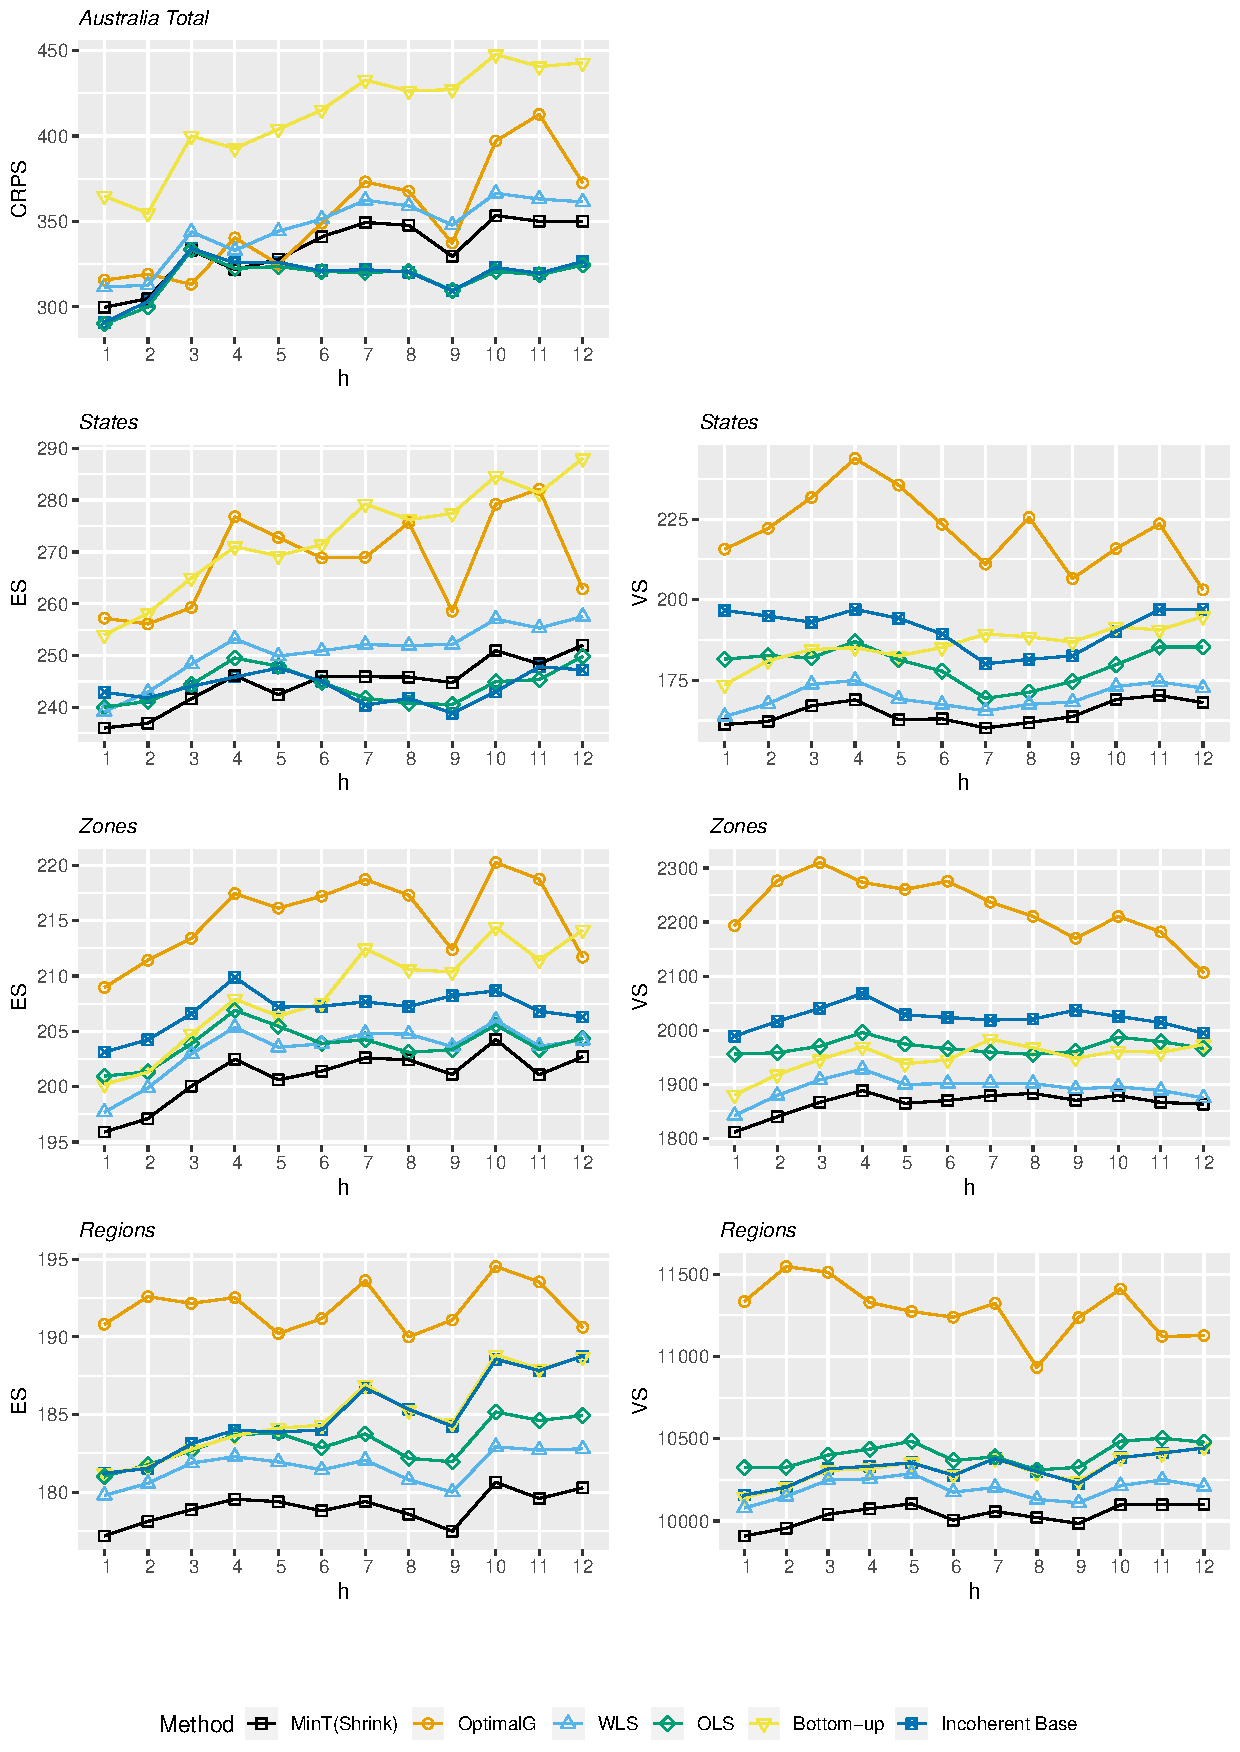
\includegraphics[width= 0.85\textwidth, height= 0.85\textheight]{RawScore_Analytical_Levels.pdf}
	\caption{Forecast accuracy results across the different levels of the Australia tourism hierarchy. CRPS results are presented for the top-level and energy and variogram scores for the levels below. A lower (higher) score indicates a more (less) accurate forecast. All results are for the analytic solution assuming Gaussian incoherent base forecasts.} \label{fig:ES-Levels}
\end{figure}

\begin{figure}
	\centering
	\small
	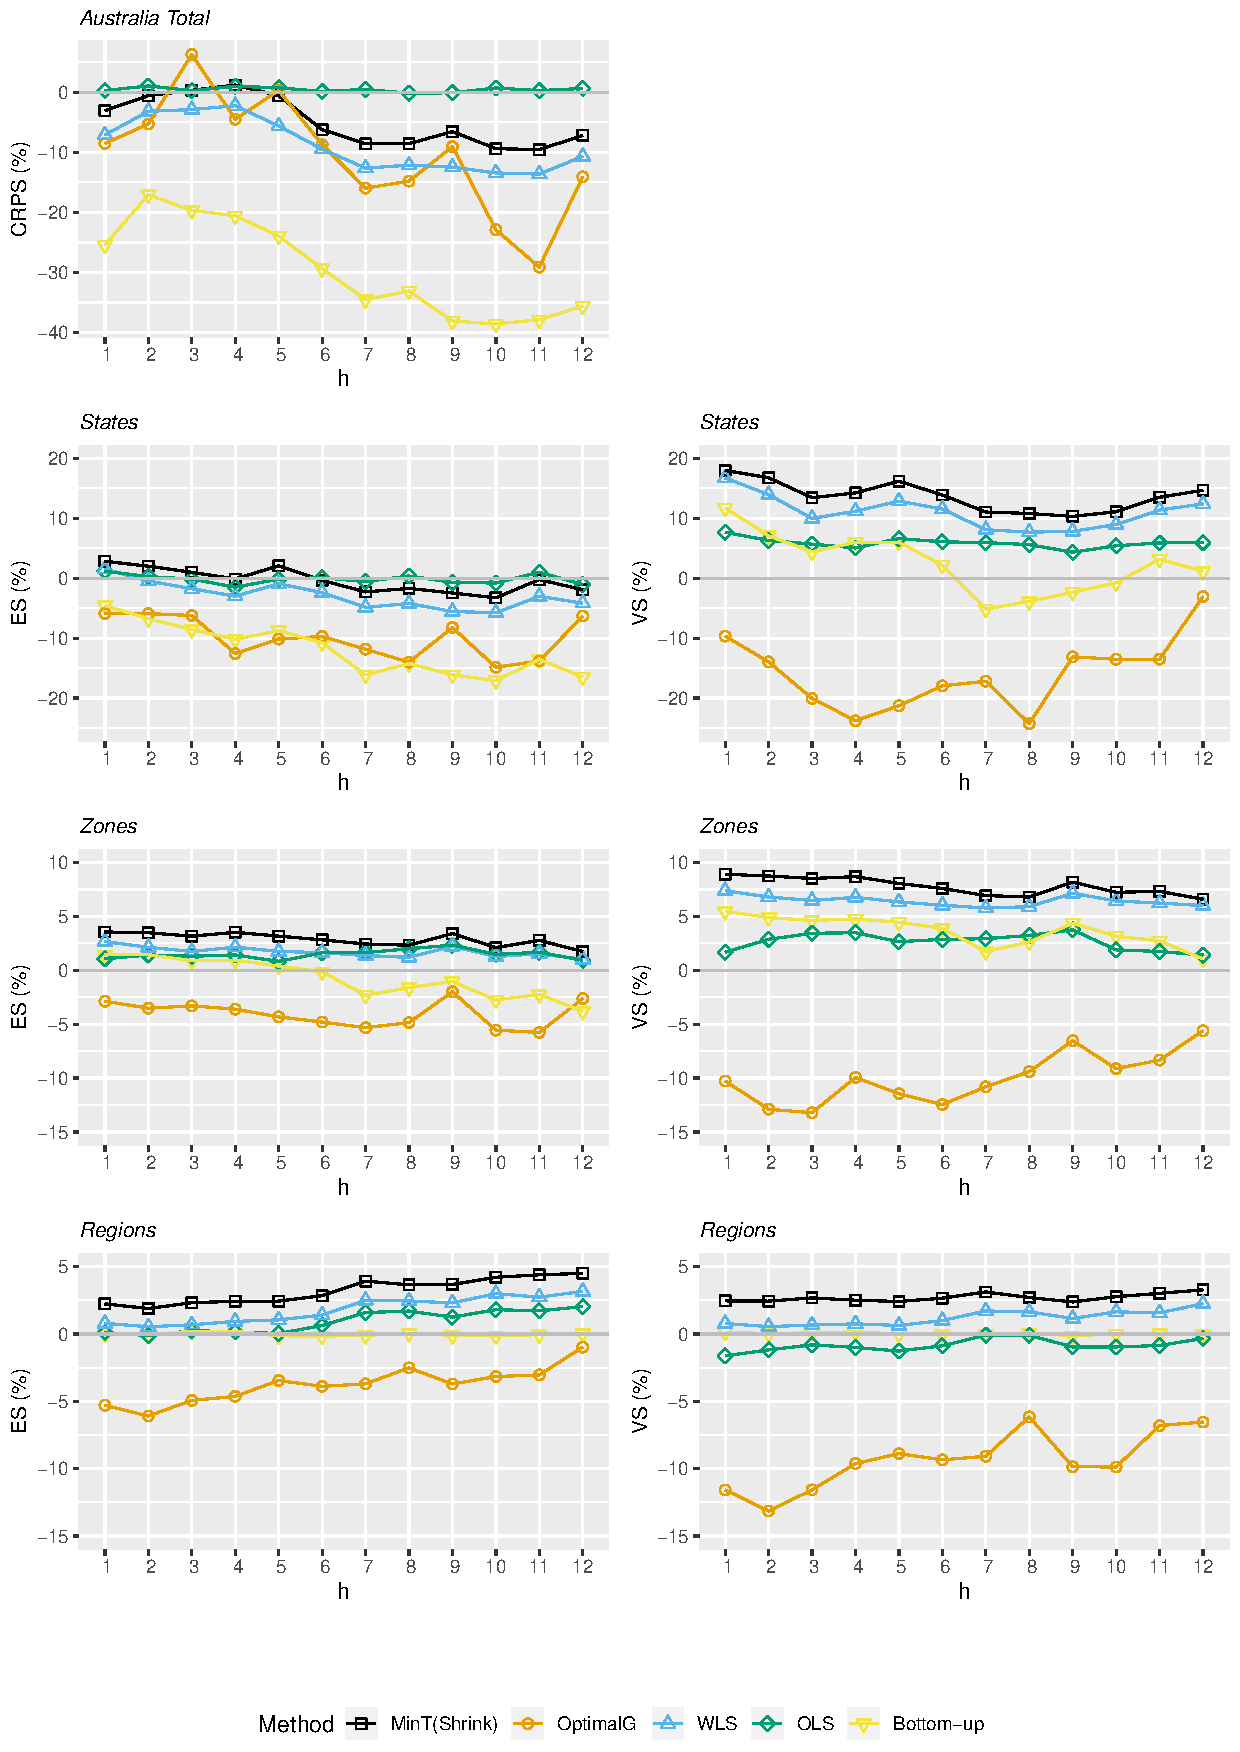
\includegraphics[width= 0.85\textwidth, height= 0.85\textheight]{SkillScore_Analytical_Levels.pdf}
	\caption{Skill scores (\%) relative to incoherent base forecasts, for the CRPS for the top-level and energy and variogram scores for the levels below for the Australia tourism hierarchy. A higher (lower) score indicates a gain (loss) in forecast accuracy relative to the incoherent base forecasts. All results are for the analytic solution assuming Gaussian incoherent base forecasts.} \label{fig:ES-SS-Levels}
\end{figure}



\begin{figure}
	\centering
	\small
	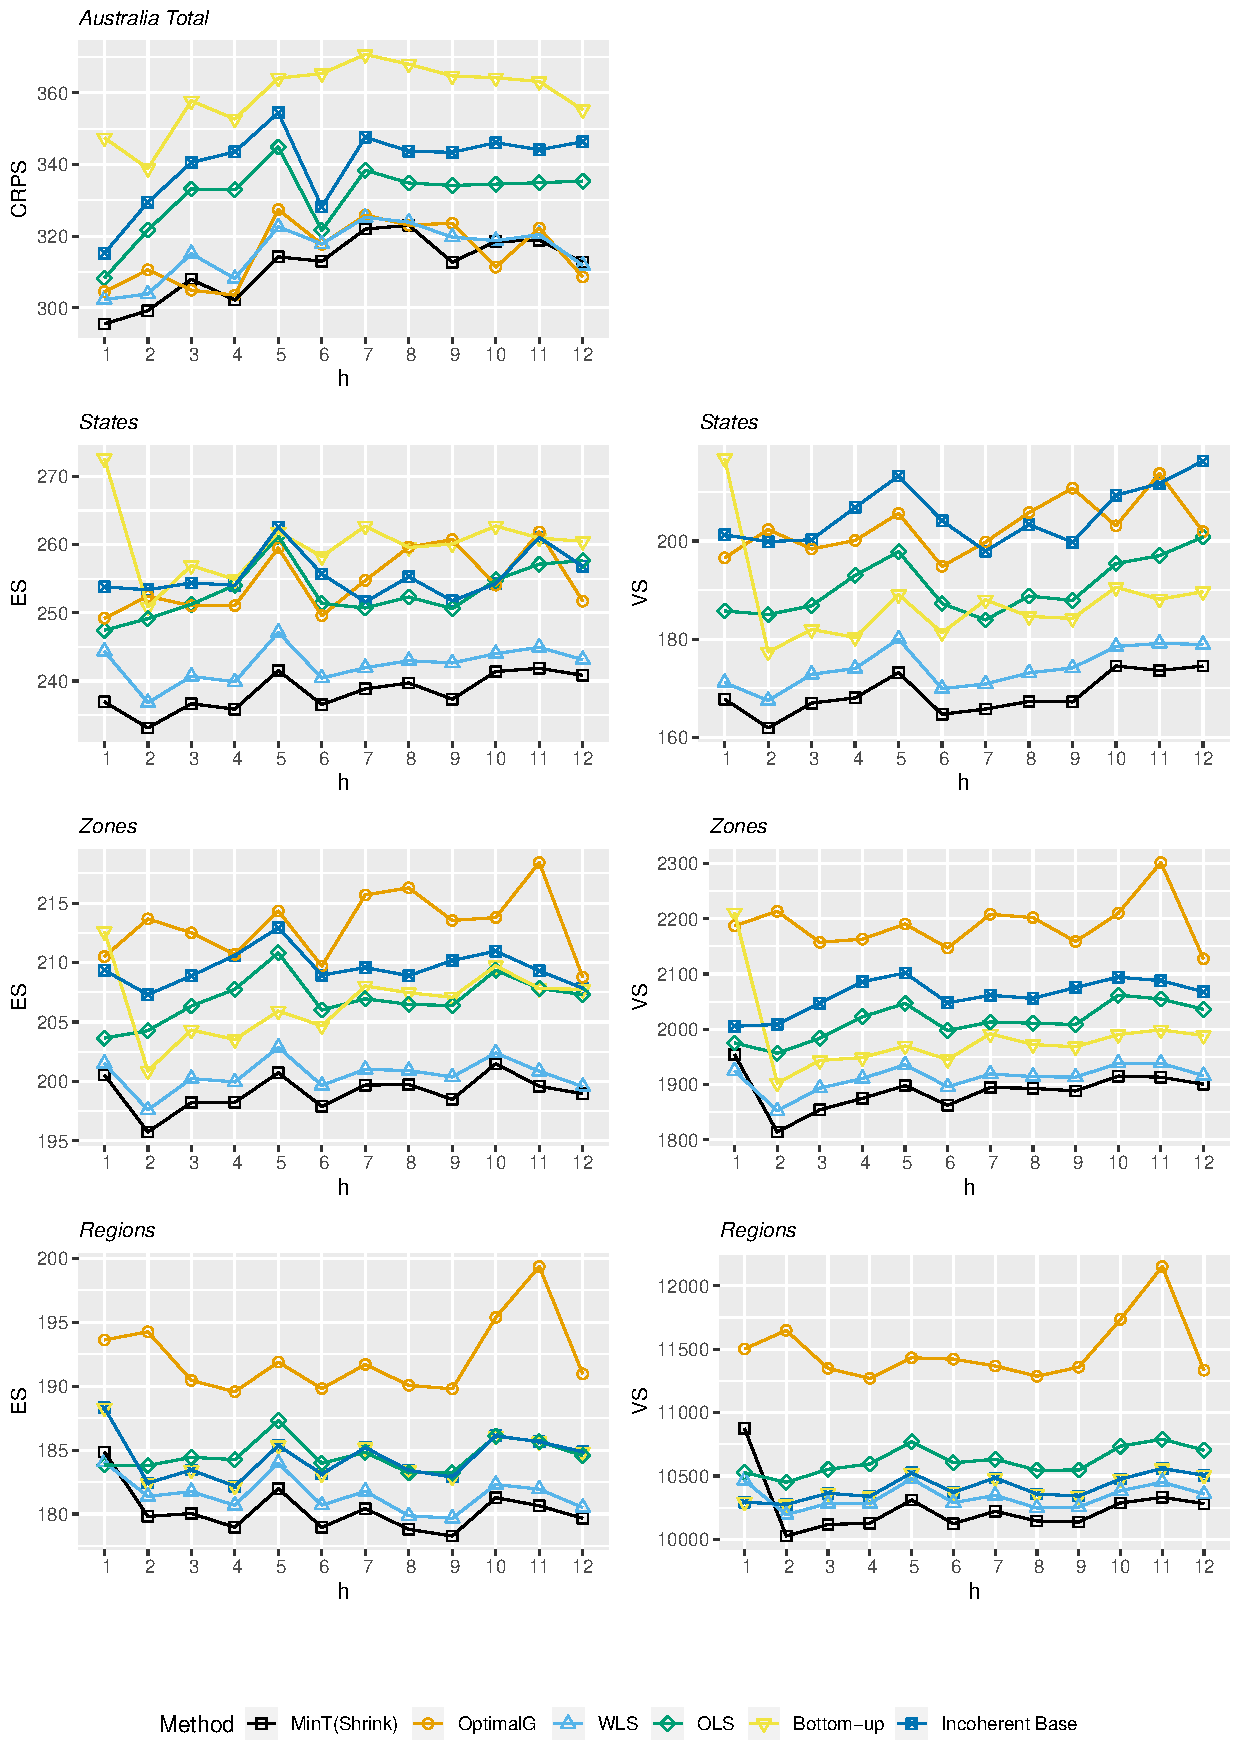
\includegraphics[width= 0.85\textwidth, height= 0.85\textheight]{RawScore_Sampling_Levels.pdf}
	\caption{Forecast accuracy results across the different levels of the Australia tourism hierarchy. CRPS results are presented for the top-level and energy and variogram scores for the levels below. A lower (higher) score indicates a more (less) accurate forecast. All results are for the sampling solution.} 
\end{figure}

\begin{figure}
	\centering
	\small
	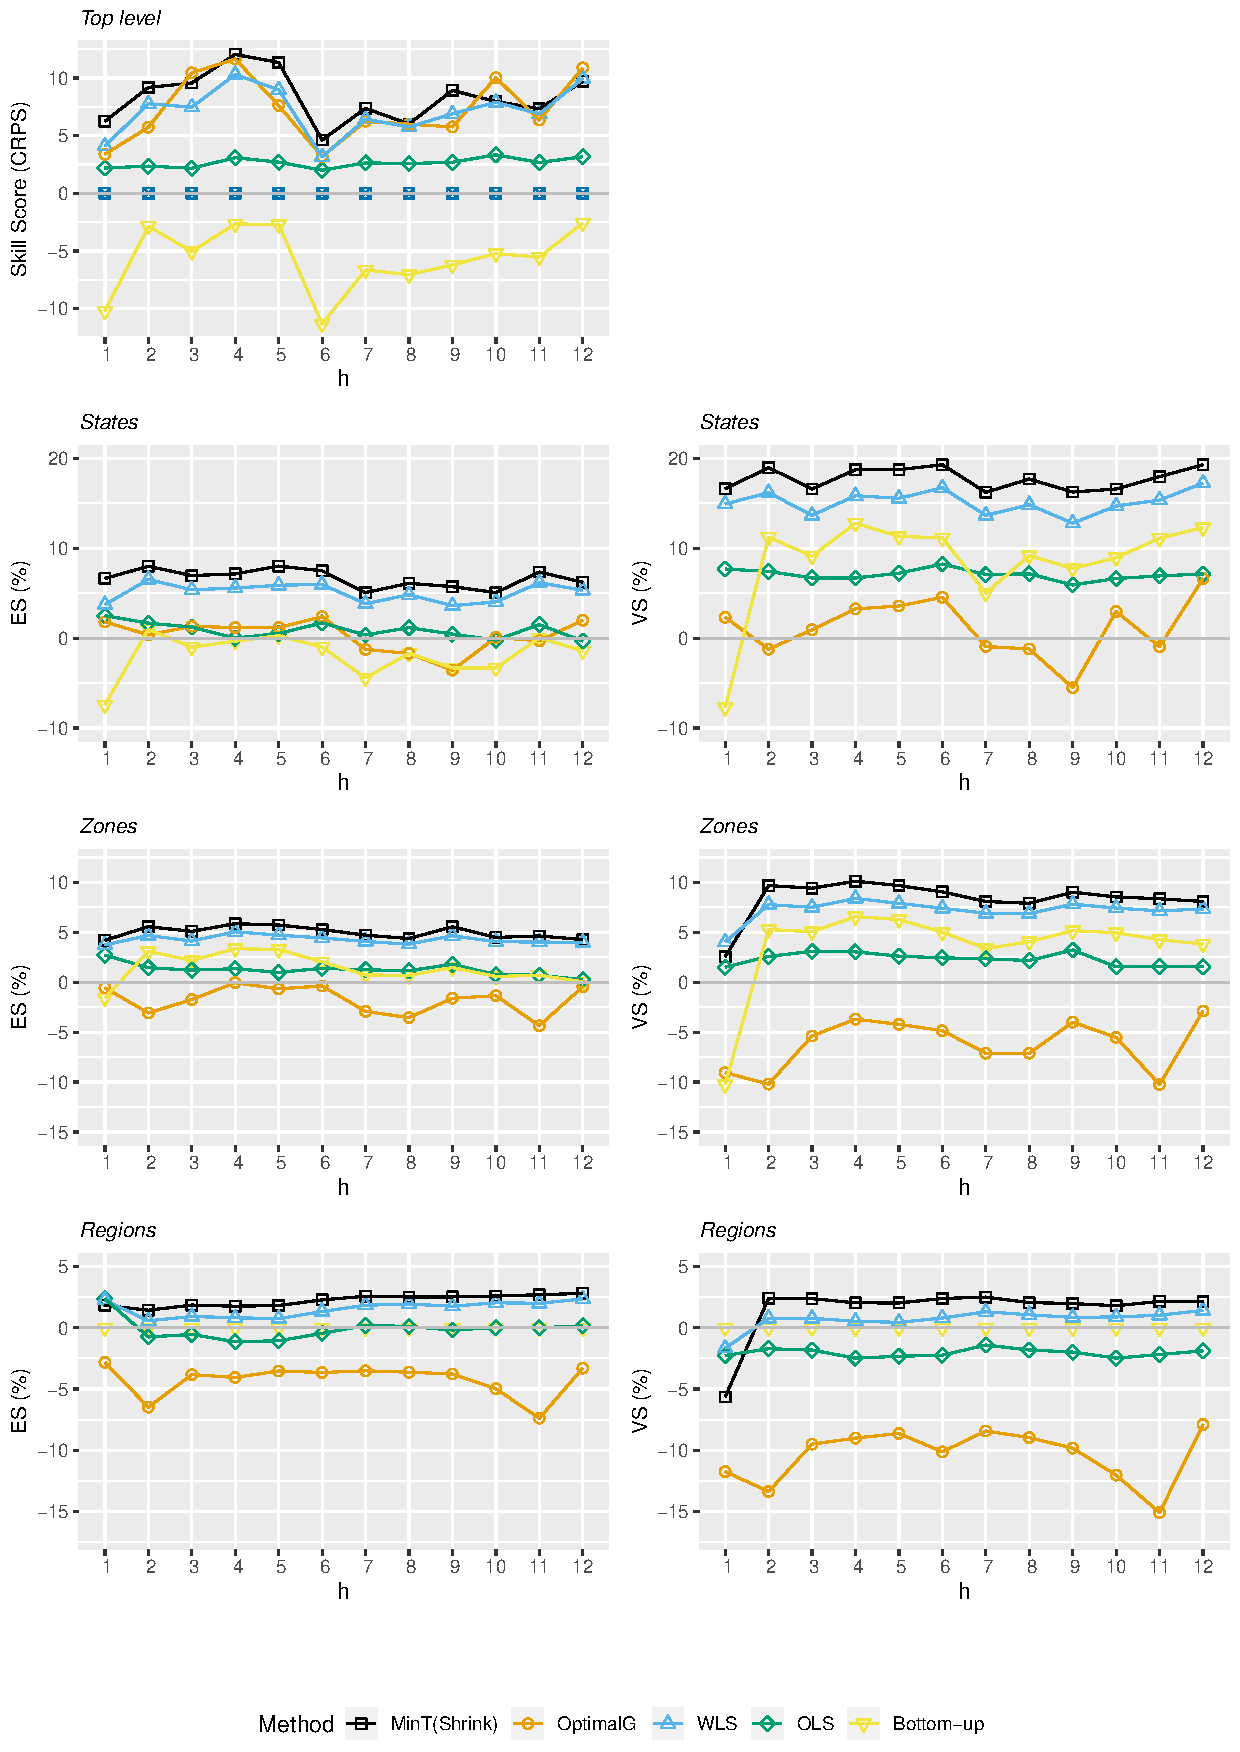
\includegraphics[width= 0.85\textwidth, height= 0.85\textheight]{SkillScore_Sampling_Levels.pdf}
	\caption{Skill scores (\%) relative to incoherent base forecasts, for the CRPS for the top-level and energy and variogram scores for the levels below for the Australia tourism hierarchy. A higher (lower) score indicates a gain (loss) in forecast accuracy relative to the incoherent base forecasts. All results are for the sampling solution.} 
\end{figure}


\end{document} 